\documentclass{birkart}
\usepackage{harvard}
\usepackage{graphics}


% THEOREM Environments (Examples)------------------------------------------
 \newtheorem{theorem}{Theorem}[section]
 \newtheorem{cor}[theorem]{Corollary}
 \newtheorem{lem}[theorem]{Lemma}
 \newtheorem{prop}[theorem]{Proposition}
 \theoremstyle{definition}
 \newtheorem{defn}[theorem]{Definition}
 \theoremstyle{remark}
 \newtheorem{rem}[theorem]{Remark}
 \newtheorem*{ex}{Example}
 \numberwithin{equation}{section}

\def\RR{\mathbb{R}}
\def\OO{\mathcal O}
\def\PP{\mathbb{P}}
\def\LL{\mathcal L}
\def\FF{\mathcal F}
\def\XX{\mathcal X}
\def\SS{\mathcal S}
\def\AA{\mathcal A}
\def\TT{\mathcal T}
\def\HH{\mathcal H}
\def\JJ{\mathcal J}
\def\argmin{\text{argmin}}
\newcommand{\Jureckova}{Jure\v{c}kov\'{a}}
\newcommand{\Hajek}{H\'{a}jek }
\newcommand{\Hardle}{H\"{a}rdle }
\newcommand{\Sidak}{\v{S}id\'{a}k }
\newcommand{\Cramer}{Cram\'{e}r}




\begin{document}
\bibliographystyle{econometrica}

\title[How to be Pessimistic]
 {How to be Pessimistic:\\ Choquet Risk and Portfolio Optimization}
%----------Author 1
\author[Bassett, Koenker, and Kordas]{Gilbert W. Bassett, Jr.}
\address{University of Illinois at Chicago}
\author{Roger Koenker} 
\address{University of Illinois at Urbana-Champaign}
\author{Gregory Kordas}
\address{University of Pennsylvania}



\thanks{Version \today. The authors would like to express their
appreciation to Steve Portnoy and Quanshui Zhao for  helpful
discussions related to this work.  }



\begin{abstract}
We review some recent developments in the theory of risk assessment.
A pessimistic decision theory emerges that replaces the subjective
probability assessments of the Savage expected utility criterion
with a Choquet expectation that accentuates the likelihood of the 
least favorable outcomes.  We show that pessimistic portfolio optimization 
may be formulated as an exercise in quantile regression.
\end{abstract}
\maketitle

\pagestyle{myheadings}
\markboth{\sc How to be Pessimistic}{\sc Bassett, Koenker, and Kordas}
 

%\vspace{5mm}
\setcounter{footnote}{0}
\renewcommand{\thefootnote}{\arabic{footnote}}


\section{Introduction}

Many economic decision problems boil down to a choice among competing
random variables.  In the \citeasnoun{vNM} and \citeasnoun{S.54} formalisms 
an investor comparing two prospects
evaluates the expected utilities of their (subjective) returns distributions:
a prospect with return distribution $F$ is preferred to another with
distribution $G$ provided that,
\[
\int_{- \infty}^\infty u(x) dF(x) \geq \int_{- \infty}^\infty u(x) dG(x) .
\]
This approach places a heavy burden on the utility function, $u(x)$,  to fully
reflect investors' attitudes toward risk, and has been called into
question by \citeasnoun{E.61} and many subsequent authors.  In reaction to
such criticism an alternative formalism, variously called 
rank-dependent, or non-additive, or Choquet
expected utility, has gradually emerged based on work of \citeasnoun{Q.81},
\citeasnoun{S.89} \citeasnoun{W.89} and others.  
See \citeasnoun{Fishburn} and \citeasnoun{Starmer} 
for valuable surveys of this work, placing it in the broader context
of other alternatives to expected utility theory.
The crucial feature of the Choquet approach 
is that it allows the investor to systematically distort the probability 
assessments underlying the Savage calculus and thereby reflect 
more nuanced attitudes toward risk and uncertainty.

Without delving deeply into technical or philosophical details, 
we will try to provide an elementary
exposition of Choquet expected utility and illustrate how it is connected
to some recent developments in risk assessment and the measurement of
inequality.  Our primary objective will be to link the rather abstract
idea of Choquet risk with a very concrete new approach to portfolio
optimization.  We will restrict attention to the case of scalar random
variables so we may write expected utility as,
\[
E u(X) = \int_{- \infty}^\infty u(x) dF(x) = \int_0^1 u(F^{-1}(t)) dt .
\]
where $F^{-1}(t) = \inf\{ x:  F(x) \geq t \}$.
%We will assume throughout that distribution functions are absolutely
%continuous with a strictly positive density on their support so
%the quantile functions we require are unambiguously defined.  This might
%be relaxed eventually.  

Now let $\nu$ be a distribution function on $[0,1]$
and define the Choquet expected utility of X as,
\[
E_\nu u(X) = \int_0^1 u(F^{-1}(t)) d\nu (t) .
\]
Obviously, for $\nu(t)=t$ we have the Savage special case.  
The {\it distortion} $\nu$ reweights the probability assessments
according to their rank order in utility.  This presumes, of course,
that utility is monotone.
The family of distortions, $\nu_\alpha (t) = \min \{t/\alpha , 1\}$ for 
$\alpha  \in [0,1]$ will play an important role. Focusing for
a moment on a single $\nu_\alpha$ we have,
\[
E_{\nu_\alpha} u(X) = \alpha^{-1} \int_0^\alpha u(F^{-1}(t))dt,
\]
and we see that -- relative to the Savage
computation of expected utility -- the probabilities of the $\alpha$ least
favorable outcomes are accentuated and the $1-\alpha$ most favorable
outcomes are discounted entirely.  
This may be interpreted as a form of investor
pessimism:  subjective probabilities are distorted to make the least
favorable events appear more likely and the most favorable events less likely.
As your gloomy aunt might put it:
``Expect the worst, and you won't be disappointed.''
The crucial feature of the Choquet expectation is that it restricts
the distortion to depend only on the rank of the events.  
Thus, in comparing two prospects that have the same ordering of events, i.e. 
random variables that differ only by monotonic transformation, we can
revert to the Savage comparison. 
Such prospects are termed {\it comonotone}. \footnote{More formally, 
two random variables, $X,Y$ are comonotone, if there exists
monotone functions $f,g$ and a random variable $U \sim U[0,1]$ such that
$X = f(U)$ and $Y = g(U)$. } 

We have, at least once, heard it objected against the Choquet view of
expected utility that the distortions of pessimism, or optimism, can
be simply accomodated into Savage's personalistic view of probability.
On this point we reserve judgement, but it seems worthwhile to recall
that Savage himself did not think so:
\begin{quote} 
I have, at least once, heard it objected against the personalistic view
of probability that, according to that view, two people might be of
different opinions, according as one is pessimistic and the other
optimistic.  I am not sure what position I would take in abstract discussion
of whether that alleged property of personalistic views would be
objectionable, but I think it is clear from the formal definition of
qualitative probability that the particular personalistic view sponsored here
does not leave room for optimism and pessimism, however these traits
may be interpreted, to play any role in the person's judgement of
probabilities.  (Savage(1954, p. 68)
\end{quote} 


\subsection{Inequality Assessment}
Measurement of inequality is closely related to risk assessment.  We can
imagine Veblen's Social Engineer trying to compare income distributions
behind the  Rawlsian veil of ignorance. 
%Again we will focus on distributions for real valued random variables.  
A classical measure of inequality is the Gini coefficient,
\[
\gamma = 1-2 \int_0^1 L (t) dt
\]
where $L(t)$ is the Lorenz function,
\[
L (t ) = \int_0^t F^{-1} (s) ds / \int_0^1 F^{-1}(s) ds
\]
As noted by \citeasnoun{Gajdos} the Gini coefficient reflects an assumption
of linearity in envy in the sense that a Pigou-Dalton transfer between
adjacent individuals at the top of the income distribution has the same
effect on the Gini as the same transfer between adjacent individuals at the 
bottom of the distribution.  There has been considerable interest in generalized
Gini coefficients that reweight the Lorenz curve according to something
other than Lebesgue measure, motivated by the idea that transfers at the
bottom of the distribution might be considered more significant.  
Clearly, the Lorenz curve is closely akin
to $\nu_\alpha$ Choquet expected utility.  
It is a linear functional of the quantile function,
and thus reweighted Gini's are representable as
Choquet expectations.  See, e.g. \citeasnoun{D.90}.

\begin{figure}
\begin{center}
\resizebox{\textwidth}{!}{
{\includegraphics{fig0.ps}}}
\end{center}
\caption{Survival Functions for a hypothetical medical treatment:
The Lehmann quantile treatment effect is the horizontal distance
between the survival curves.  In this example consideration of
the mean treatment effect would slightly favor the (dotted) treatment curve, 
but the pessimistic patient might favor the (solid) placebo curve.} 
\end{figure}

\subsection{Quotidian Risk}
In the everyday drudgery of decision making --  should I rob that bank?
should I agree to surgery tomorrow? -- we are often confronted with complicated
problems of risk assessment.  In evaluating the risk of medical interventions
we find it helpful to consider the Lehmann quantile treatment effect,
see \citeasnoun{KG.01}.  Suppose that as a patient facing surgery you are told
that in the absence of surgery you face the survival distribution
$S_0 (t) = 1 - F_0 (t)$ while if you elect to have the surgery you face
$S_1 (t) = 1 - F_1 (t)$.  In the absence of any further information, 
it is reasonable to evaluate the two prospects on the basis of the
quantile treatment effect function,
\[
\delta ( t ) = F_0^{-1}(t) - F_1^{-1}(t) = S_1^{-1} (1-t)  - S_0^{-1} (1-t) . 
\]
Integrating, we obtain,
\[
\mu_\delta = \int_0^1 \delta(t)dt,
\]
the mean treatment effect, the average difference in survival times
between the control and treatment regimes.  The dedicated follower of Savage
might simply evaluate the two prospects by computing this quantity,
and choose accordingly.  

Suppose that survival prospects
with and without the surgery are as illustrated in Figure 1.  With 
the surgery there is about a 15 percent chance of a full recovery
and a greatly extended lifetime, but with very high probability your prospects
are actually better without the surgery.  Let's suppose that the upper 
tail probabilities are such that mean survival time is slightly better under
the treatment.  Does this constitute a compelling case for the surgery?
Clearly the optimist would say, ``I'm feeling lucky and I like my chances
of falling into that upper 15  percent, bring on the surgeon.''
But the pessimist might say instead,
``I'll take my chances with the placebo.  There is
only a 1 in 7 chance the surgery is going to do me any good.'' 
Is there something irrational about the latter view?  One might say
that a decision like this all depends upon how the patient discounts
the future.  Perhaps the pessimist just lives for the moment, and the
optimist is able to imagine, and act upon, the prospect of the
rosy scenario on the distant horizon.  Decision theory has focused most
of its attention on this nonlinearity of tastes over the horizontal
axis:  wealth should be transformed into utility, survival times
should be discounted.  Then we can simply compute expectations.
But even after such discounting, we suggest, rational
preferences may still admit some element of nonlinearity on
the vertical axis of probabilities.  


\vspace{3mm}
In the next section we provide an overview of some recent work on
risk assessment and its relation to Choquet expected utility.
The third section links the resulting notion of Choquet risk to
the optimization problem
underlying quantile regression.  And it is shown that 
portfolio optimization methods based on minimizing Choquet risk
can be easily implemented using existing algorithms for quantile
regression.  

\section{Choquet Risk}

In response to regulatory concerns in the finance sector there has been
intensive recent interest in the question of how to evaluate portfolio risk. 
An influential paper in this literature is \citeasnoun{ADEH.99}, 
which provides an axiomatic foundation for ``coherent'' risk measures.
\begin{defn}
(Artzner {\it et al})
For real valued random variables $X \in \XX$ on $(\Omega , \AA)$ 
a mapping $\varrho: \XX \rightarrow \RR$ is called a coherent risk measure 
if it is:
\begin{enumerate}
\item Monotone:  $X,Y \in \XX, \mbox{with} \; X \leq Y \Rightarrow \varrho(X) \geq \varrho (Y)$.
\item Subadditive:  $X,Y,X+Y \in \XX$,  
		$\Rightarrow \varrho(X+Y) \leq \varrho (X) + \varrho (Y)$.
\item Linearly Homogeneous:  For all $\lambda \geq 0$ and $X \in \XX$, 
		$\varrho(\lambda X) = \lambda \varrho (X)$.
\item Translation Invariant:  For all $\lambda \in \RR$ and $X \in \XX$, 
		$\varrho(\lambda + X) = \varrho (X) - \lambda $.
\end{enumerate}
\end{defn}
These requirements rule out many of the conventional measures of risk
traditionally used in finance.  In particular, measures based on second moments
including the standard deviation are ruled out, as are quantile based
measures like the value at risk.  A measure of risk that has gained
considerable recent prominence in the wake of these findings is,
\[
\varrho_{\nu_\alpha} (X) =  - \alpha^{-1}  \int_0^\alpha F^{-1}(t) dt .
\]
Variants of $\varrho_{\nu_\alpha} (X)$ have been suggested 
under a variety of names:  expected shortfall
(\citeasnoun{AT.01}), conditional VaR (\citeasnoun{RU.00}),
tail conditional expectation (\citeasnoun{ADEH.99}).\footnote{
The terminology of Uryasev and Rockafellar seems somewhat unfortunate, 
since it seems to suggest that cVaR is a conditional quantile rather
than a conditional mean.}
For the sake of brevity we will call 
$\varrho_{\nu_\alpha} (X)$ the $\alpha$-risk
of the random prospect $X$.  Clearly, $\alpha$-risk is simply the
negative Choquet $\nu_\alpha$ expected return.\footnote{ 
We note in passing, in the hope that it may be deemed relevant at 
some later point,
that elsewhere in the probability literature, e.g. \citeasnoun{H.98} and
\citeasnoun{Hobson}, the random variable $X^*$ whose quantile function is,
\[
F_{X^*}^{-1}(u) = (1-u)^{-1} \int_u^1 F_X^{-1} (v)dv
\]
is called the Hardy-Littlewood transform of $X$.  Obviously, the $\alpha$-risks
constitute the negative Hardy-Littlewood transform of the random variable $-X$.} 
Having defined $\alpha$-risk in this way, it is natural to consider the
criteria: $\varrho_{\nu_\alpha} (X) - \lambda \mu (X)$, or
$\mu(X) - \lambda \varrho_{\nu_\alpha} (X).$
Minimizing the former criterion may be viewed
as minimizing risk subject to a constraint on mean return;
maximizing the latter criterion may be viewed as maximizing return
subject to a constraint on $\alpha$-risk.
Several authors, including
\citeasnoun{D.90}, \citeasnoun{RU.00}, and \citeasnoun{JK.01},
have suggested criteria of this form as alternatives to the classical
Markowitz criteria in which $\alpha$-risk is replaced by the standard
deviation of the random variable $X$.
Since $\mu(X) = \int F_X^{-1} (t) dt = - \varrho_1 (X)$ these criteria
are special cases of the following more general class.
\begin{defn} A risk measure $\varrho$ will be called {\it pessimistic}
if, for some probability measure $\varphi$ on $[0,1]$,
\[
\varrho (X) = 
\int_0^1 \varrho_{\nu_\alpha} (X) d \varphi (\alpha).
\]
\end{defn}
To see why such risk measures are pessimistic,
note that by the  Fubini Theorem we can write,
\[
\varrho (X) = - \int_0^1 \alpha^{-1} 
\int_0^\alpha F^{-1} (t) dt d \varphi (\alpha)
= - \int_0^1 F^{-1} (t) \int_t^1  \alpha^{-1}  d \varphi (\alpha) dt.
\]
In the simplest case, we can take $\varphi$ as a sum of  point masses, 
say $d\varphi = \sum_i \varphi_i \delta_{\tau_i}$ with
$\varphi_i >0$ and $\sum \varphi_i = 1$ and noting that 
\[
\int_t^1 \alpha^{-1} \delta_\tau (\alpha) d \alpha = \tau^{-1} I(t < \tau),
\]
we can write 
\[
\varrho (X) = 
\int_0^1 \varrho_{\nu_\alpha} (X) d \varphi (\alpha)
= - \int_0^1  F^{-1} (t) \gamma(t) dt 
\]
%approximate general measures, $\varphi$, by piecewise linear ones,
%and the resulting Choquet risks for these approximates have a piecewise
%constant (histogram-like) density weighting,
where $\gamma(t) = \sum_i \varphi_i \tau_i^{-1} I(t < \tau_i)$.
Positivity of the point masses, $\varphi_i$,
assures that the resulting density weights are decreasing, so the
resulting distortion in probabilities acts to accentuate the implicit
likelihood of the least favorable outcomes.
Such preferences are clearly ``pessimistic''.  

Following \citeasnoun{K.01} we will impose some additional 
regularity conditions on $\varrho$:
\begin{defn}
Let $\LL^\infty$ denote the space of all bounded 
real-valued random variables on $(\Omega, \FF, \PP)$ with $\PP$ non-atomic.
A map $\varrho: \LL^\infty \rightarrow \RR$ is a {\it regular}
risk measure if: 
\begin{enumerate}
\item[i.]  $\varrho$ is law invariant, i.e. $\varrho(X)=\varrho(Y)$ if
$X,Y \in \LL^\infty$ have the same probability law.
\item[ii.]  $\varrho$ satisfies the Fatou property, 
i.e. if $\{ X_n \}_{i=1}^n \subset \LL^\infty$ are uniformly bounded and 
converge to $X$ in probability 
then $\varrho (X) = \lim\inf_{n \rightarrow \infty} \varrho(X_n)$. 
\item[iii.]  $\varrho$ is comonotone, i.e. 
$X,Y \in \LL^\infty$ comonotone implies that
$\varrho (X+Y) = \varrho (X)  + \varrho (Y) $. 
\end{enumerate}
\end{defn}

The first two regularity conditions impose a relatively weak form of
continuity, while the third condition refines slightly the the subadditivity
property.  We can now succinctly reformulate the main representation 
result of \citeasnoun{K.01}.
\begin{theorem}
A regular risk measure is coherent if and only if it is pessimistic.
\end{theorem}
\vspace{3mm}
One could, of course, also consider a more general class of Choquet risk 
measures,
\[
\varrho (X) = - \int F_X^{-1} (t) d \nu (t),
\]
for distribution functions $\nu$ on $[0,1]$.  
Pessimistic risk measures correspond to concave $\nu$, assigning
decreasing density on the interval $[0,1]$.
``Optimistic'' risk measure would have convex $\nu$, 
thus reweighting more favorable outcomes more heavily, and discounting
the likelihood of less favorable eventualities.
It is quite plausible to consider $\nu$ that are concave in the lower tail
and convex in the upper tail as a way to rationalize 
buying flight insurance for a trip to Las Vegas.
%the commonly observed willingness to purchase
%insurance and buy lottery tickets.
\citeasnoun{Q.93}  provides an excellent discussion
of possible motivations for these possibilities, 
so we will resist the temptation to delve further into them. 
Instead,  we now turn to a description of an empirical approach to portfolio
optimization based on {\it pessimistic} risk measures.

\section{How to be Pessimistic}

Empirical strategies for optimizing $\alpha$-risk lead immediately into the 
realm of quantile regression.  Let $ \rho_\tau(u) = u(\tau - I(u<0))$ 
denote the ``check function'' of \citeasnoun{KB.78} and consider the
problem,
$$
\min_{\xi \in \RR}  E\rho_\alpha (X-\xi) .
$$
We know that any $\xi$ solving this problem is an $\alpha$th quantile of the
random variable $X$.  
Evaluating at the minimizer, $\xi_\alpha$ we find that
minimizing the usual $\alpha$-quantile objective function
is equivalent to evaluating the sum of expected return
and the (Choquet) $\alpha$-risk of $X$, and then multiplying by $\alpha$.

\begin{theorem}
Let $X$ be a real-valued random variable with $EX = \mu < \infty$, then
\[
\min_{\xi \in \RR}  E\rho_\alpha (X-\xi) = \alpha ( \mu + \varrho_{\nu_\alpha} (X)).
\]
\end{theorem}
\begin{proof}
Noting that,
\[
E\rho_\alpha (X-\xi) = \alpha ( \mu - \xi ) - 
\int_{-\infty}^\xi (x - \xi)dF_X (x),
\]
is minimized when $\xi_\alpha = F_X^{-1} (\alpha)$, we have,
\[
E\rho_\alpha (X-\xi_\alpha ) = \alpha  \mu + \alpha \varrho_{\nu_\alpha} (X).
\]
\end{proof}

The empirical analogue of $\alpha$-risk can thus be formulated as
\[
\hat \varrho_{\nu_\alpha} (x) = (n \alpha)^{-1} \min_{\xi \in \RR}
\sum_{i=1}^n \rho_\alpha (x_i - \xi) -  \hat \mu_n
\]
where $\{ x_i : i=1,... , n\}$ constitutes a random sample on $X$, and
$\hat \mu_n$ denotes an estimator of $EX=\mu$, presumably, $\bar x_n$.
Of course $\hat \varrho_{\nu_\alpha} (x)$ 
could easily be defined in a seemingly more direct manner, but the value of the
proposed optimization formulation becomes apparent as soon as 
we begin to consider {\it portfolios} of assets.  Let $Y=X^\top \pi$
denote a portfolio of assets comprised of $X=(X_1 , ... , X_p)^\top$
with portfolio weights $\pi$.  Suppose we observe a random sample
$\{x_i = (x_{i1}, ... , x_{ip}): i = 1, ... , n \}$ and we wish to consider
portfolios minimizing
\begin{equation}\label{arisk}
\min_\pi \varrho_{\nu_\alpha} (Y) - \lambda \mu (Y).
\end{equation}
This is evidently equivalent to simply minimizing 
$ \varrho_{\nu_\alpha} (Y) $ subject to a constraint on mean return.
We will impose the additional constraint that the portfolio weights $\pi$
sum to one, and reformulate the problem as,
\[
\min_\pi \varrho_{\nu_\alpha} (X^\top \pi) \; s.t. \; \mu (X^\top \pi) = \mu_0,
\; 1^\top \pi =1.
\]
Taking the first asset as numeraire we can write the sample analogue of
this problem as 
\begin{equation}\label{arho}
\min_{(\beta,\xi) \in \RR^p } \sum_{i=1}^n 
\rho_{\alpha} (x_{i1} - \sum_{j=2}^p (x_{i1}-x_{ij})\beta_j -\xi)
\; s.t. \; \bar x^\top \pi (\beta) =\mu_0,
\end{equation}
where $\pi(\beta) = (1-\sum_{j=2}^p \beta_j , \beta^\top )^\top$.
It is easy to verify that the solution is invariant to the choice of
the numeraire asset.  At the solution, $\hat \xi$ is the
$\alpha$th sample quantile of the chosen portfolio's returns distribution.
The required return constraint implicitly corresponds to a particular $\lambda$
in the original specification \eqref{arisk}.  Note that we have not (yet)
imposed any further constraints on the portfolio weights $\beta$, but
given the linear programming form of the problem \eqref{arho} it would
be straightforward to do so.

The problem posed in \eqref{arho} is (almost) a conventional quantile
regression problem.  The only idiosyncrasy is the mean return constraint,
but it is easy to impose this constraint by simply adding a single pseudo
observation to the sample consisting of response $\kappa (\bar x_i - \mu_0)$
and design row 
$\kappa ( 0, \bar x_1 - \bar x_2, ... , \bar x_1 - \bar x_p )^\top$.
For sufficiently large $\kappa$ we are assured that the constraint will be
satisfied.  Varying $\mu_0$ we obtain an empirical $\alpha$-risk frontier.

\begin{figure}
\begin{center}
\resizebox{\textwidth}{!}{
{
\includegraphics{fig1.ps}}}
\end{center}
\caption{Four Asset Densities for Example:  
We will construct portfolios comprised of four independent
asset returns with marginal densities illustrated above.}
\end{figure}

\begin{figure}
\begin{center}
\resizebox{\textwidth}{!}{
{
\includegraphics{fig2.ps}}}
\end{center}
\caption{The $\alpha$-risk-return frontier:  
For the four artificial asset returns series 
we compute the risk-return frontier according to \eqref{arho} in panel
b.  The portfolio weights as functions of the required mean
return are depicted in Panel c.} 
\end{figure}

\begin{figure}
\begin{center}
{\includegraphics{fig3.ps}}
\end{center}
\caption{Mean-variance vs. $\alpha$-risk portfolio returns:  
Based on the data of example 1 we illustrate the estimated density of
portfolio returns for the optimal mean-variance portfolio and the optimal
$\alpha$-risk portfolio for required mean return of .07.
Note the the solid curve representing the $\alpha$-risk returns has
better performance than the dotted mean-variance density in both tails. } 
\end{figure}



{\bf Example}  Our first illustration of the approach will be 
based on a small artificial dataset.  We generate {\it independent}
returns on 4 assets with marginal densities illustrated in Figure 2.
Solving \eqref{arho} with various values of $\mu_0$, we obtain portfolios
with weights illustrated in Figure 1c and the risk-return frontier 
appearing in Figure 4.  How do these portfolios compare to the mean-variance
portfolios of the classical theory for this data?  In Figure 3 we compare
the returns densities of the optimal $\alpha$-risk portfolio with the optimal
mean variance portfolio performance for two different levels of required
mean return.  The four assets should be seen as two pairs:  a lower pair
consisting of a normal density with mean .04 and standard deviation .02
and a left skewed reversed $\chi_3^2$ density with the same mean and
standard deviation, and an upper pair consisting of a normal density with
mean return .08 and standard deviation .05, and a right skewed $\chi_3^2$
density with the the same mean and standard deviation.  
The $\alpha$-risk portfolios tend to prefer the right skewed asset
and disdain the left skewed one.  For example at required mean return
.07, the $\alpha$-risk  portfolio puts weight .55 on right skewed asset
and only .11 weight on its normal counterpart,
while the mean-variance portfolio places equal weight, .33, 
on both. {\hfill{ \rule{2mm}{2mm}}}

%{\bf Example 2.}  Our second illustration constitutes a mild perturbation
%of the previous example, but the conclusions change quite dramatically.
%We illustrate the new densities of the four independent candidate assets
%in Figure 4; they are rescaled versions of the prior densities with more
%separation between the performance of the more dispersed, higher return
%densities.  Repeating the previous exercise, if we compute the mean
%variance frontier for portfolios comprised of these assets we obtain
%the first panel of Figure 5, however the $\alpha$ risk frontier with
%$\alpha =.1$ appearing in the second panel indicates that returns can
%be increased without bound, while at the same time  
%{\it decreasing} $\alpha$-risk.  What is happening?  A look at the resulting
%$\alpha$-risk portfolios reveals that as the required mean return is
%pushed up, the investor puts larger and larger weight on the positively skewed
%asset and this produces portfolio returns distributions that
%are increasingly skewed to the right, having  larger and larger mean,
%but also having smaller and smaller $\alpha$-risk.  The mean-variance
%portfolios have a similarly skewed character as required mean return is
%increased, however using standard deviation of the portfolio returns
%as a risk measure views upside risk as just as dangerous as down side
%risk.  This accounts for the observed effect  that in the mean variance
%frontier risk increases with the mean return.  {\hfill{ \rule{2mm}{2mm}}}

Although the $\alpha$-risks provide a convenient one-parameter family of
coherent risk measures, they are obviously rather simplistic.  As we have
already suggested, it is natural to consider weighted averages of
$\alpha$-risks:
\[
\varrho_\nu (X) = \sum_{k=1}^m \nu_k \varrho_{\nu_{\alpha_k}} (X).
\]
Where the weights, $\nu_k : k=1, ... , m$, are positive and sum to one.
This risk criterion can also be easily implemented empirically
extending the formulation in \eqref{arho}
\begin{equation}\label{nurho}
\min_{(\beta,\xi) \in \RR^{p+m} } \sum_{k=1}^m \sum_{i=1}^n \nu_k
\rho_{\alpha} (x_{i1} - \sum_{j=2}^p (x_{i1}-x_{ij})\beta_j -\xi_k)
\; s.t. \; \bar x^\top \pi (\beta) =\mu_0.
\end{equation}
The only new wrinkle is the appearance of $m$ distinct intercept parameters
representing the $m$ estimated quantiles of the returns distribution of the
chosen portfolio.  In effect we
have simply stacked $m$ distinct quantile regression problems on top
of one another and introduced a distinct intercept parameter for each of
them, while constraining the portfolio weights to be the same for each
quantile.  Since the $\nu_k$ are all positive, they may passed inside
the $\rho_\alpha$ function to rescale the argument.  The statistical
theory of such constrained quantile regression estimators is discussed
in \citeasnoun{K.84}.

\section{Extensions}
There are many loose ends and topics for future research.  An important
byproduct of the quantile regression formulation of the $\alpha$-risk
portfolio optimization problem is the attendant statistical inference
provided.  This is most straightforward in the case of the simple
$\alpha$-risk objective function, but can be extended to the general
case of weighted sums of $\alpha$-risks.  We hope to consider these
issues in future work.  There are also many other possible refinements
including the incorporation of additional constraints.  Upper and lower
bounds on the positions held in the portfolio would often be
appropriate, and would be easy to implement, as would shrinkage
of portfolio weights toward some {\it a priori } portfolio.  Most
importantly, it is necessary to explore, prod, and test the Choquet
approach on realistic applied problems.

The expected utility theory of von Neumann and Morgenstern is firmly
embedded in the {\it zeitgeist} of modern decision theory.  It has
withstood more than a half century of severe criticism, whether 
a viable alternative theory can be built on the foundations of Choquet
expectation remains an open question.  But it is a question that
deserves further investigation.

\bibliography{port}

\end{document}
